\documentclass[a4paper,12pt]{article}

\usepackage[top=2cm, bottom=2cm, left=2cm, right=2cm]{geometry}
\usepackage{amsmath}
\usepackage{amssymb}
\usepackage{graphicx} 
\usepackage{caption}
\usepackage{dsfont}
\usepackage{verbatim}
\usepackage{pdfpages}
\usepackage{subfig}

\renewcommand{\thepart}{}
\renewcommand{\thesection}{\arabic{section}}
\renewcommand{\thesubsection}{\arabic{section}.\arabic{subsection}}

%-------------------------------------------------------------------------------
\begin{document}

%Include cover
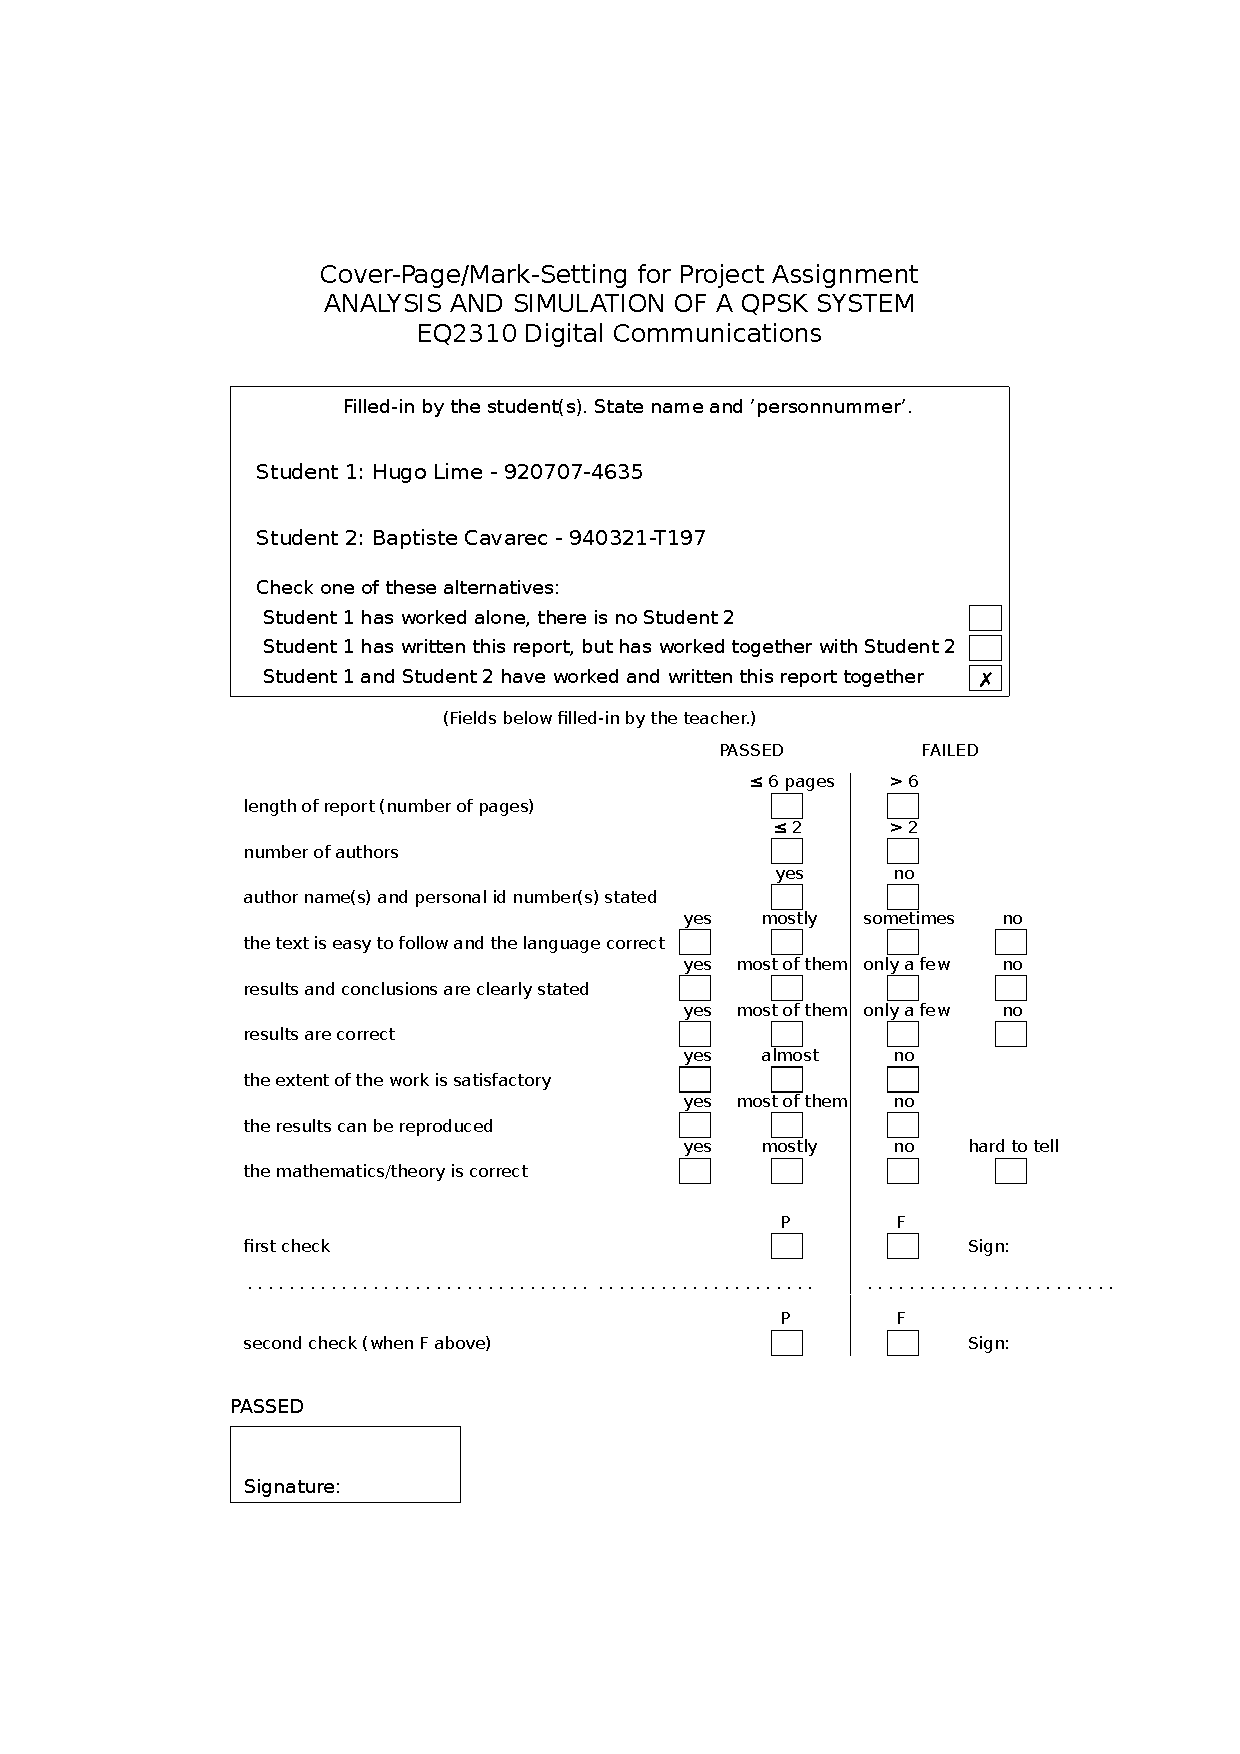
\includepdf[pages={1}]{Cover_filled.pdf}
\newpage

%Abstract
\section*{Abstract}
Throughout this project, we investigate the influence of multiple parameters in a simulated QPSK radio communication channel.
First, we simulate the evolution of the bit error rate regarding the signal-to-noise ratio in a perfectly synchronized environment. 

Then we study how synchronization and phase estimation affects the BER and the behavior of these algorithms under AWGN and lastly the influence of the training sequence.

In a last part, we examine the deterioration of BER due to a phase increase and how it can be reduced with differential demodulation.

%-----------------------------------------------------------------------------------
%Partie 1
\section{Ideal Bit Error Rate (BER) performances}

\subsection{Exact expression}
\begin{figure}[ht!]
\centering
\begin{center}
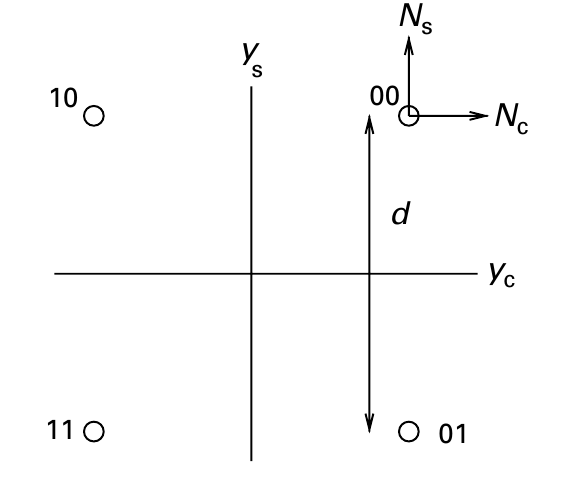
\includegraphics[scale=0.20]{Gray_coded_QPSK.png}
\caption{Gray coded bitmap from \cite{Madhow}}
\end{center}
\end{figure}
The exact expression of the BER is given by \cite{Madhow} and can easily be derived as:
\begin{equation}
p_{b}=Q(\sqrt{\frac{2E_{b}}{N_{0}}})
\end{equation}

\subsection{Simulation results and comparison}
In order to simulate an environment with perfect synchronization, we forced the value of $t_{samp}$. This value is corresponding to the number of samples coming from the guards bits and the delay caused by the matched filter. We also set the phase offset to $0$.
\begin{figure}[ht!]
\centering
\begin{center}
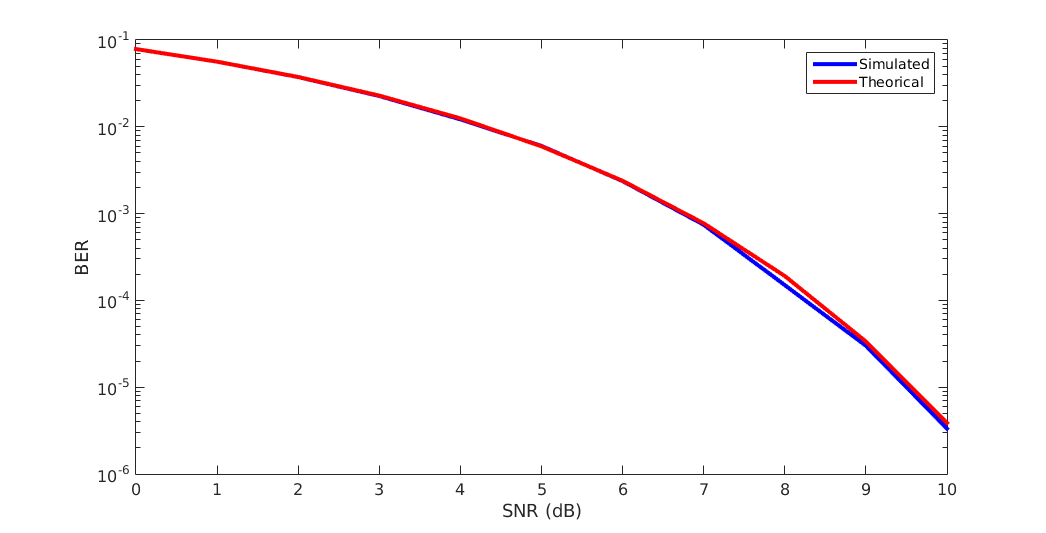
\includegraphics[scale=0.30]{BER_Exact-Sim.png}
\caption{BER comparison}
\label{BER}
\end{center}
\end{figure}
As shown in Figure \ref{BER}, the simulated values are very similar to the theoretical ones. However, for very high SNR, the BER is so small that our testing set (here 300 blocks of 1000 data bits) is not large enough to be relevant.

%-----------------------------------------------------------------------------------
%Partie 2
\newpage
\section{Non-ideal synchronization and phase estimation}
\subsection{Influence of time and phase estimation on the BER}
In order to see the influence of time, we picked a SNR of $5dB$. Then we created errors in synchronization and phase estimation to see how it modifies the BER.

\begin{figure}[ht]
\begin{minipage}[c]{.45\linewidth}
\begin{center}
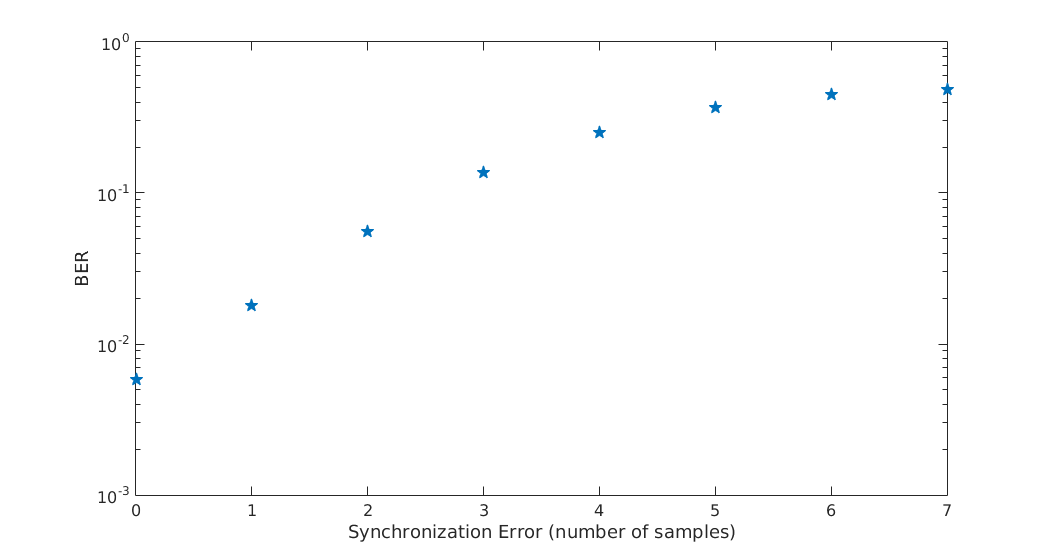
\includegraphics[scale=0.35]{BER_SyncError.png}
\caption{BER with synchronization errors}
\label{BER_sync}
\end{center}
\end{minipage}
\hfill
\begin{minipage}[c]{.45\linewidth}
\begin{center}
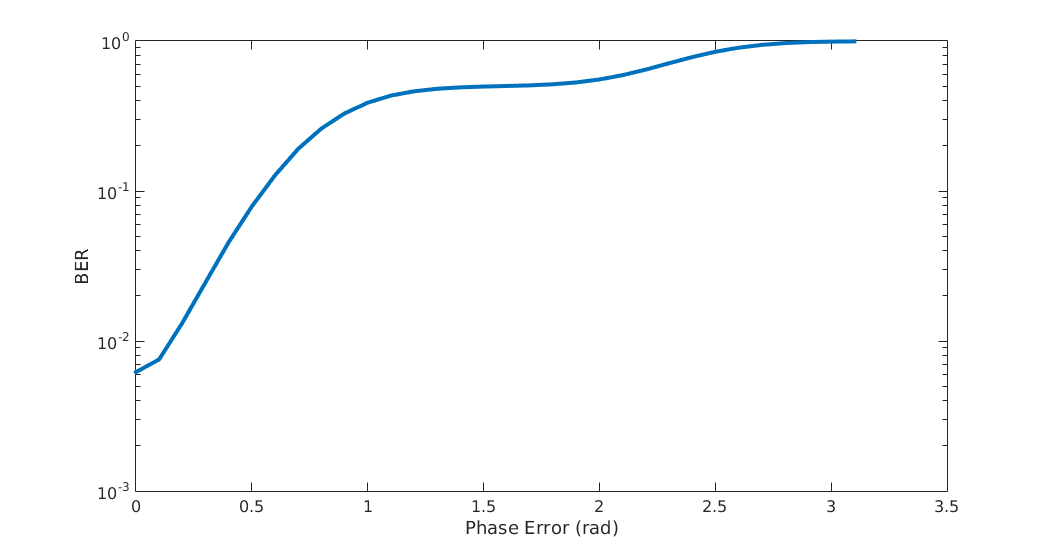
\includegraphics[scale=0.35]{BER_PhaseError.png}
\caption{BER with phase errors}
\label{BER_phase}
\end{center}
\end{minipage}
\end{figure}

Figure \ref{BER_sync} shows that one single error in the synchronization is catastrophic, the BER is multiplied by 2. With a shift of 2 samples, the BER is 10 times higher.\\

Figure \ref{BER_phase} shows that phase estimation can greatly increase the BER. However, for small error (typically less than 0.1 rad) the loss is acceptable. For a better understanding of the influence of the phase error on the BER, one can look at the constellation on Fig.~\ref{Constellation}. One can see that when the noise power increases, a lot of samples are detected near a border of a decision region. Therefore, an error in phase estimation can easily move the sample in a wrong region thus creating detection errors.

\begin{figure}[ht]
\subfloat[$SNR=0$]{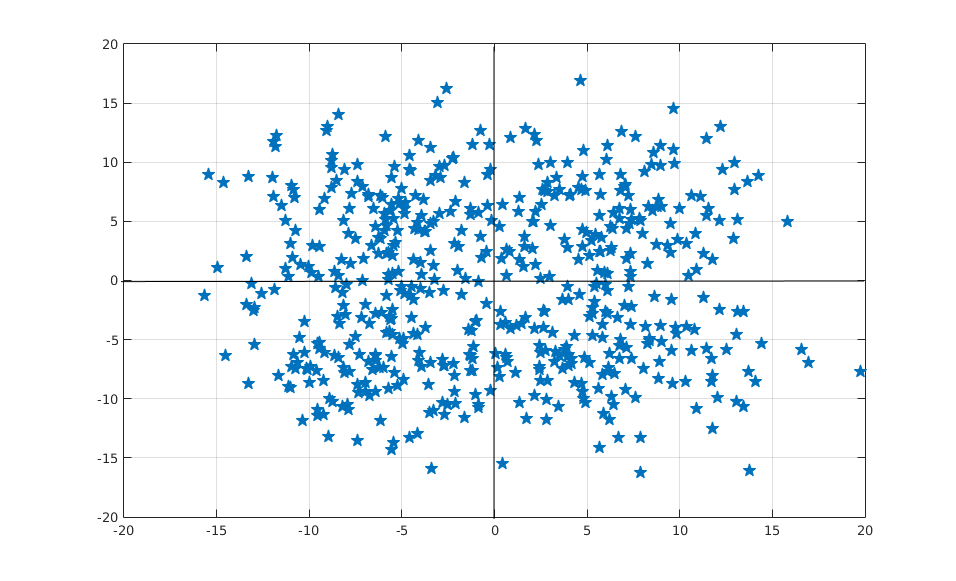
\includegraphics[width=0.35\textwidth]{Constellation_SNR0.png}} 
\subfloat[$SNR=5$]{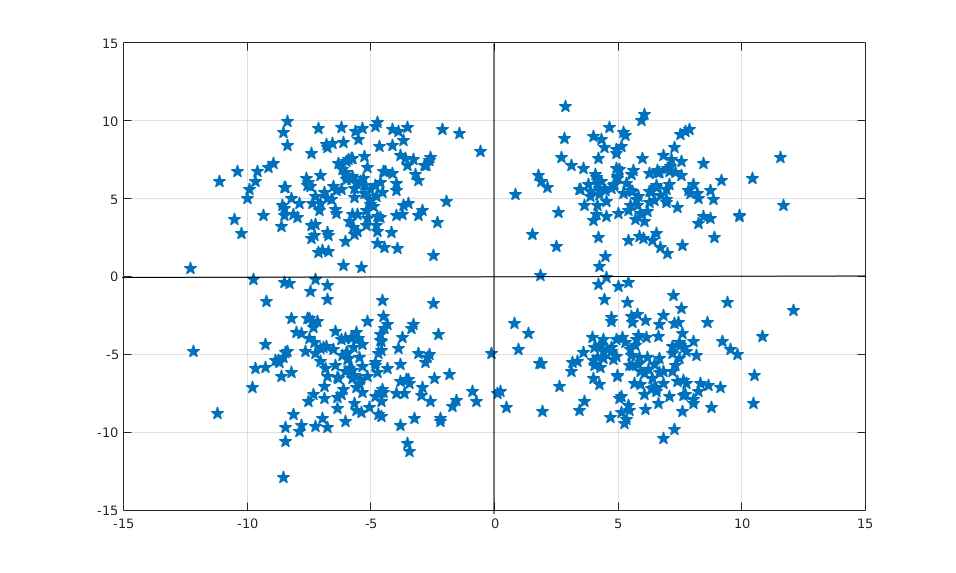
\includegraphics[width=0.35\textwidth]{Constellation_SNR5.png}} 
\subfloat[$SNR=10$]{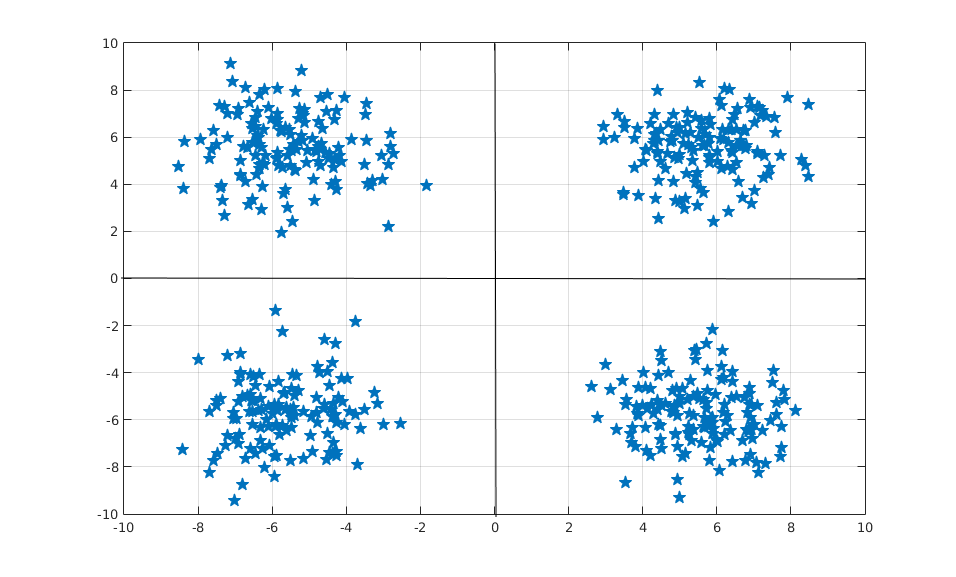
\includegraphics[width=0.35\textwidth]{Constellation_SNR10.png}} 
\caption{Constellation Diagrams}
\label{Constellation}
\end{figure}


\subsection{Synchronization and phase estimation under AWGN}
In this part we implemented the recommended synchronization algorithm (maximum cross-correlation between the filtered signal and a copy of the training sequence). Fig.~\ref{SE} shows that this algorithm is very resilient to the noise. For a reasonable SNR, errors never occur. However, one should take into account that we used a small window (around 6 symbols) centered on the real value. In a real environment we would need another system to position the window (like a power detector). \\

In order to estimate the phase, we searched for the angle that would minimize the norm of the difference between the rotated signal and the training sequence. We can see on Fig.~\ref{PE} that the estimate is quite sensible to noise. But, as stated before, a phase error of less than 0.1 rad has a reasonable effect on the BER. It could be improved by using another algorithm, or a phase-locked loop.


\begin{figure}[ht]
\begin{minipage}[c]{.45\linewidth}
\begin{center}
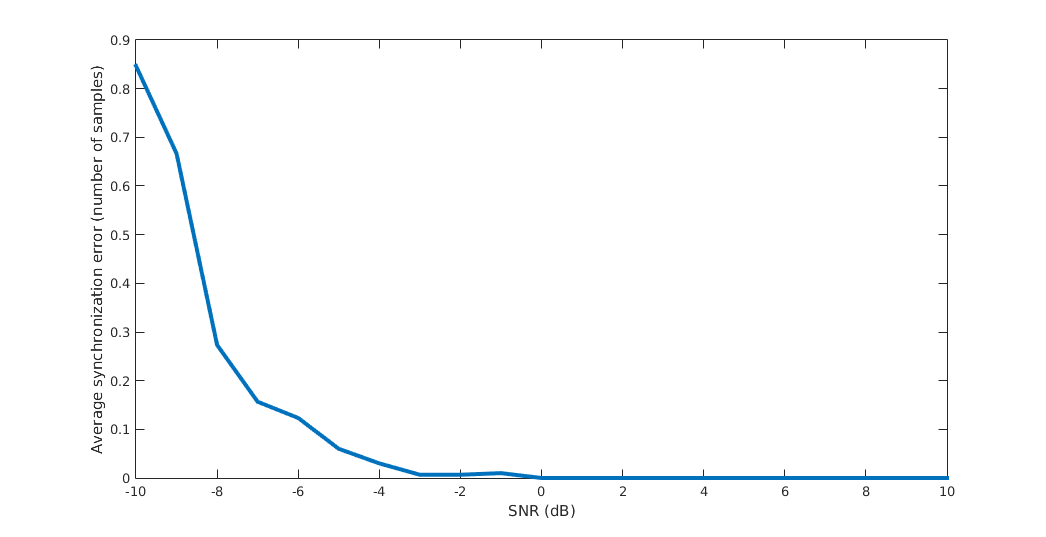
\includegraphics[scale=0.35]{SynError.png}
\caption{time estimation error}
\label{SE}
\end{center}
\end{minipage}
\hfill
\begin{minipage}[c]{.45\linewidth}
\begin{center}
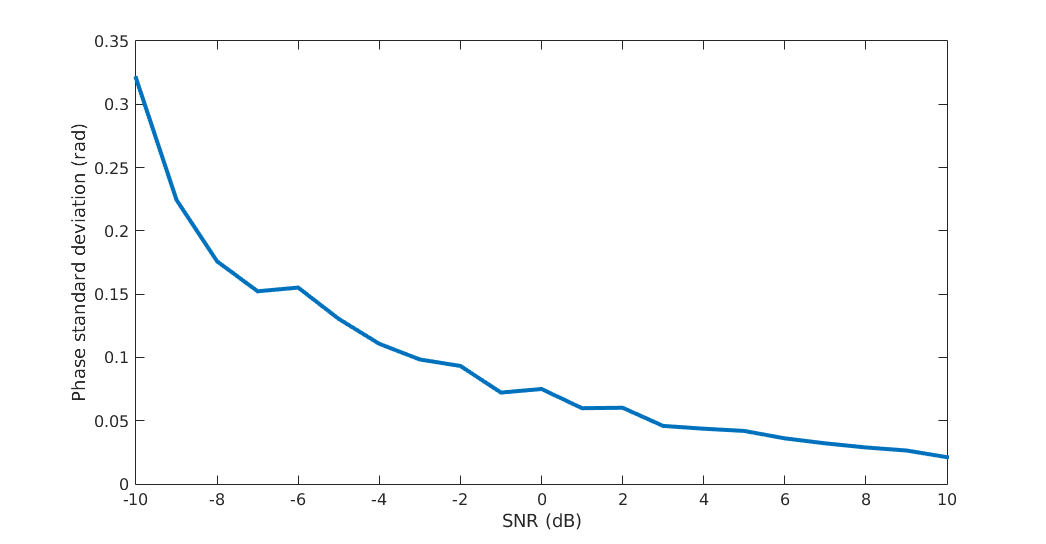
\includegraphics[scale=0.35]{PhaseError.png}
\caption{Phase estimation error}
\label{PE}
\end{center}
\end{minipage}
\end{figure}

\subsection{Influence of the training sequence}

We computed the synchronization and phase estimation errors when changing the number of training bits at a fixed SNR of 0. Fig.~\ref{TSE} shows that with a training sequence of more than 20 bits, we have less than 10\% chance of having a synchronization error.\\

For the phase estimation, if we want less than 0.1 rad deviation, as we concluded before, we need at least 50 training bits. With a fixed sequence of 1000 data bits, this would corresponds to a 5\% overhead.

\begin{figure}[ht]
\begin{minipage}[c]{.45\linewidth}
\begin{center}
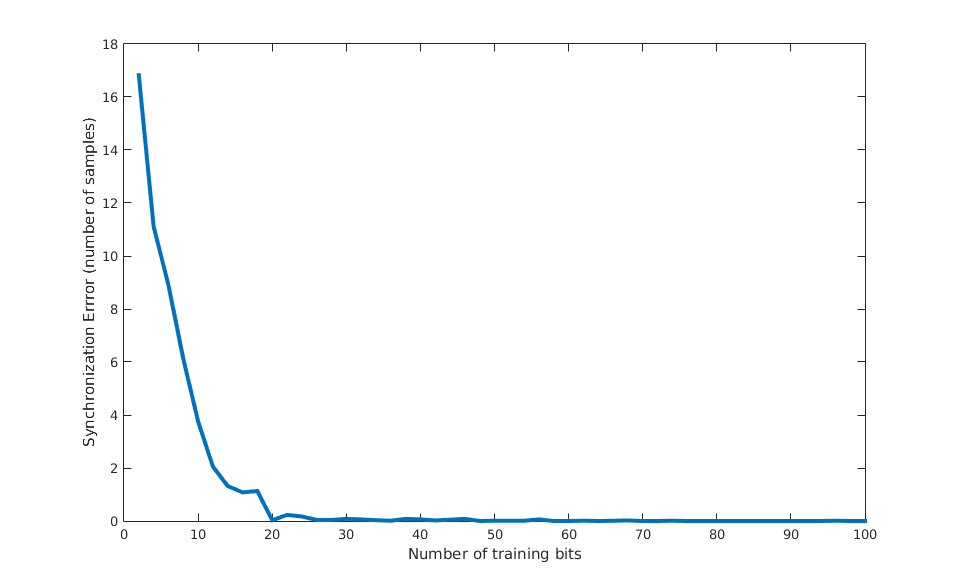
\includegraphics[scale=0.35]{Training_sync.png}
\caption{time estimation error}
\label{TSE}
\end{center}
\end{minipage}
\hfill
\begin{minipage}[c]{.45\linewidth}
\begin{center}
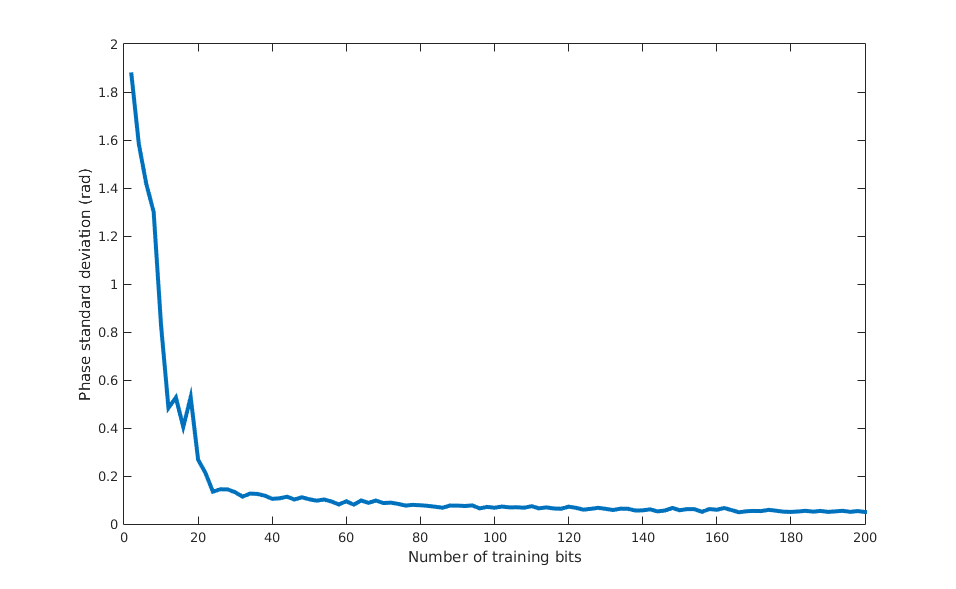
\includegraphics[scale=0.35]{Training_phase.png}
\caption{Phase estimation error}
\label{TPE}
\end{center}
\end{minipage}
\end{figure}

To improve the training sequence, we need to find one that has an autocorrelation function that is similar to a Dirac. To do this, we tested a number of random training sequences for which we computed its autocorrelation function. Then we chose the one that had the autocorrelation function most similar to a Dirac. Fig.~\ref{train} shows that for a small training sequence it can improve a little the performances of the synchronization.

\begin{figure}[ht!]
\subfloat[10 bits]{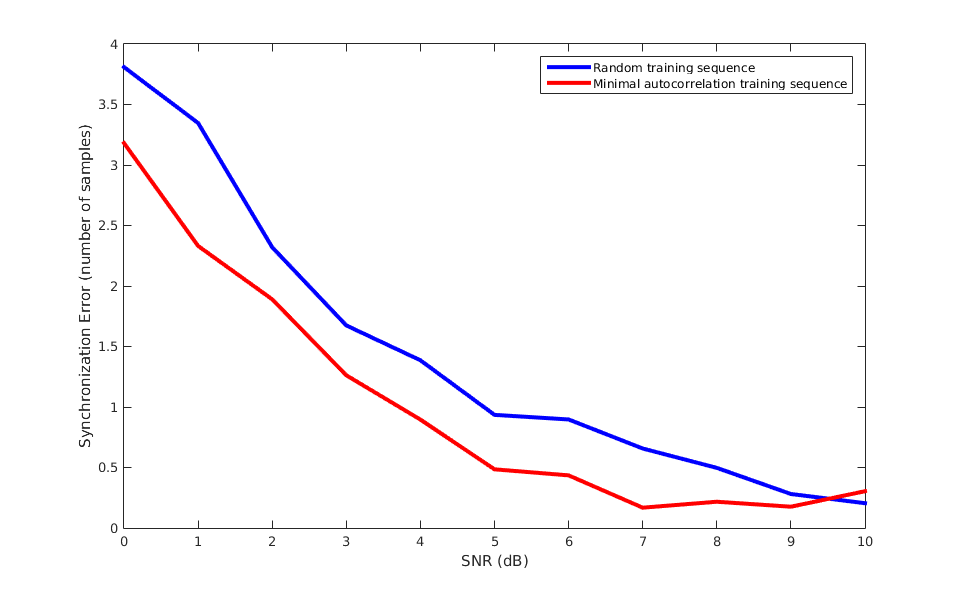
\includegraphics[width=0.55\textwidth]{Training_seq10.png}} 
\subfloat[20 bits]{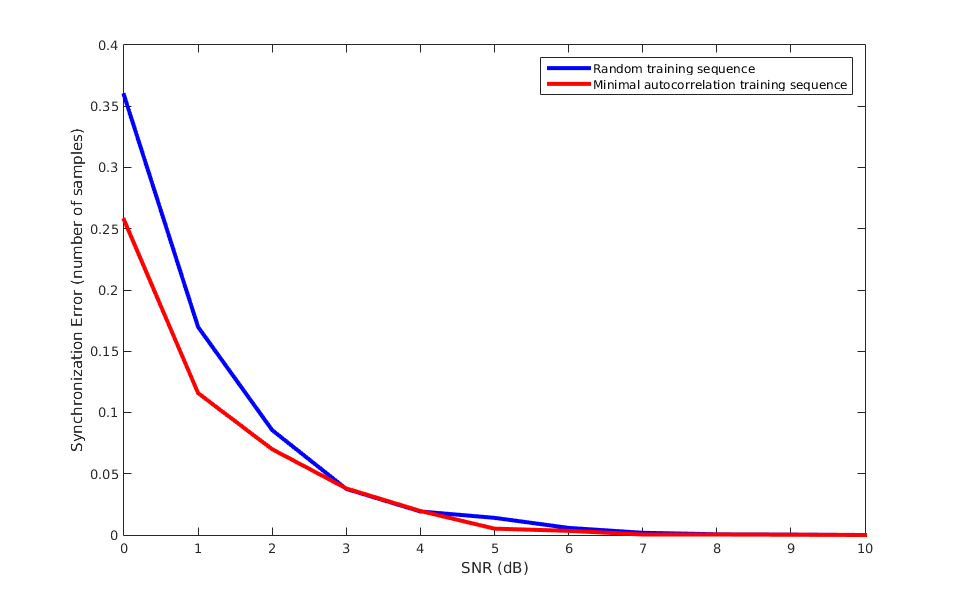
\includegraphics[width=0.55\textwidth]{Training_seq20.png}}  
\caption{Difference between random and chosen training sequence}
\label{train}
\end{figure}

%-----------------------------------------------------------------------------------
%Partie 2
\newpage
\section{Differential modulation}
\subsection{Influence of a linear phase increase}
First, we added a linear phase increase during the transmission of the block. This phase varies from $0$ to $\frac{\pi}{4}$. It is a modelisation of a small frequency offset on the local oscillator. Here we chose 50 training bits in order to satisfy previous requirements. With this phase increase, we can expect the phase detection to select a correct phase for the training bits. However, as the phase increase along the data symbol sequence, more and more errors will occur. For the last symbol, the $\frac{\pi}{4}$ phase shift should result in a 50\% probability of error a QPSK channel.\\

Fig.~\ref{BERphase} shows that such a phase increase greatly deteriorate the channel performances.

\begin{figure}[ht!]
\centering
\begin{center}
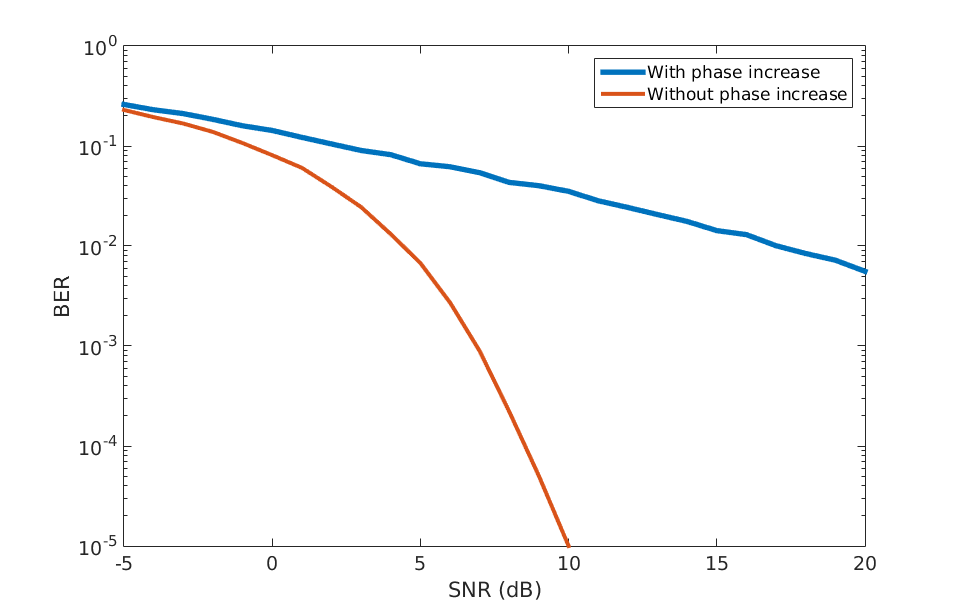
\includegraphics[scale=0.50]{BER_phase_increase.png}
\caption{BER comparison under phase increase}
\label{BERphase}
\end{center}
\end{figure}

\subsection{Differential modulation/demodulation}
In order to alleviate the phase increase effect, we can think to implement a differential modulator. Such a demodulation scheme would only rely on the phase shift from the previous symbol to detect the transmitted bits instead of the phase shit from the first symbol of the block. We can expect this to greatly alleviate the phase shift increase as in our model, this phase increase is slow so the phase is almost constant between two symbols.\\
Fig.~\ref{BERphase2} shows that, as expected, the differential modulation solves this issue for high SNR. We can also note that differential QPSK under phase increase gives worse BER than QPSK without the phase increase. It could still be interesting to solve this frequency offset in another way.



\begin{figure}[ht!]
\centering
\begin{center}
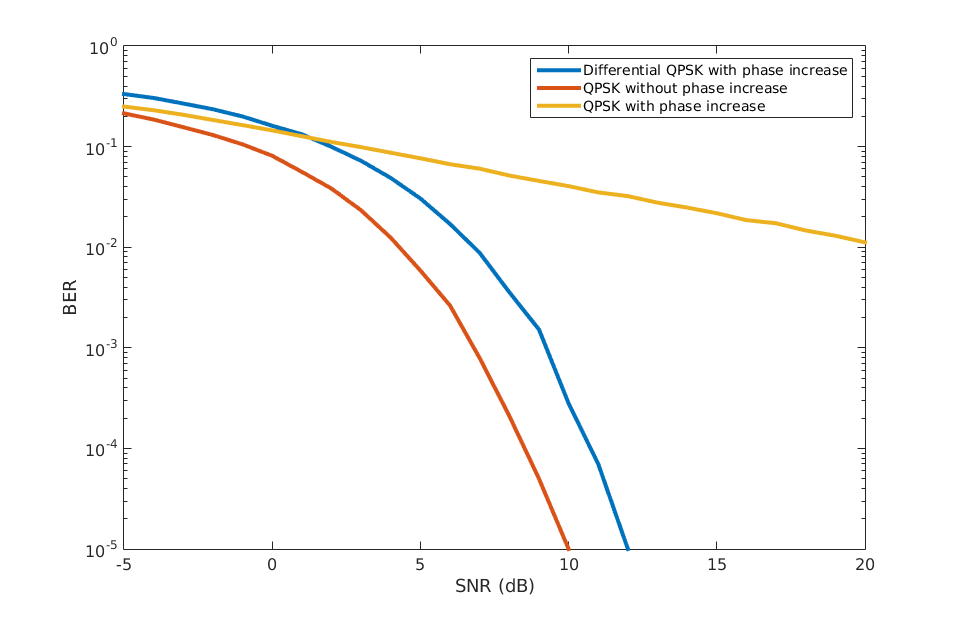
\includegraphics[scale=0.55]{BER_phase_increase2.png}
\caption{Differential modulation performances}
\label{BERphase2}
\end{center}
\end{figure}

%---------------------------------------------------------------------------------
%Conclusion
\section*{Conclusion}
To conclude this analysis and simulation of a QPSK signal, we can say that we were able to simulate a basic QPSK channel composed of a transmitter and a receiver. The results from these simulations allowed us to verify basic results of QPSK communication. Moreover, we dealt with synchronization and phase estimation which are common issues of wireless communication and we made basic test to see how differential modulation can solve some of this problems.\\

This study, however, only used a simple AWGN channel. Further research on QPSK communication should focus on modeling and simulating more complex channels with fading.

%References
\bibliographystyle{plain}
\bibliography{report_biblio}

%---------------------------------------------------------------------------------------
%Appendix
\appendix

\section*{Matlab code}
In this appendix we would only add functions we created and implemented for this project,the two last functions : diff\_qpsk and diff\_detect  are the functions we created in order to implement differential modulation. More information on our project can be found on our github repository : github.com/BaptCav/ProjetsDigitalCom-SignalProcessing/tree/master/Digital\%20Communications
\subsection*{qpsk.m}
\begin{verbatim}
function d = qpsk(b)
% d = qpsk(b)
%
% Map the bits to be transmitted into QPSK symbols using Gray coding. The
% resulting QPSK symbol is complex-valued, where one of the two bits in each
% QPSK symbol affects the real part (I channel) of the symbol and the other
% bit the imaginary part (Q channel). Each part is subsequently PAM
% modulated to form the complex-valued QPSK symbol. The energy per QPSK
% symbol is normalized to unity.
%
% The mapping resulting from the two PAM branches are:
%
% complex part (Q channel)
%         ^
%         |
%  10 x   |   x 00   (odd bit, even bit)
%         |
%  -------+------->  real part (I channel)
%         |
%  11 x   |   x 01
%         |
%
%
%
% Input:
%   b = bits {0, 1} to be mapped into QPSK symbols
%
% Output:
%   d = complex-valued QPSK symbols

%Add a 0 the end if the sequence is not even
if(mod(length(b),2)==1)
    b=[b,0];
end

N= length(b);
d=zeros(1,N/2);
for i =1:(N/2)
    if(b(2*i-1)==1 && b(2*i)==1) %11
        d(i)= -1-1i;
    elseif(b(2*i-1)==0 && b(2*i)==1) %01
        d(i)=1-1i;
    elseif (b(2*i-1)==0 && b(2*i)==0) %00
        d(i)=1+1i;
    else %10
        d(i)=1i-1;
    end
end
d=1/sqrt(2)*d;

\end{verbatim}

\subsection*{sync.m}
\begin{verbatim}
function t_samp = sync(mf, b_train, Q, t_start, t_end)
% t_samp = sync(mf, b_train, Q, t_start, t_end)
%
% Determines when to sample the matched filter outputs. The synchronization
% algorithm is based on cross-correlating a replica of the (known)
% transmitted training sequence with the output from the matched filter
% (before sampling). Different starting points in the matched filter output
% are tried and the shift yielding the largest value of the absolute value
% of the cross-correlation is chosen as the sampling instant for the first
% symbol.
%
% Input:
%   mf            = matched filter output, complex baseband, I+jQ
%   b_train       = the training sequence bits
%   Q             = number of samples per symbol
%   t_start       = start of search window
%   t_end         = end of search window
%
% Output:
%   t_samp = sampling instant for first symbol


bqpsk=qpsk(b_train);
n = length(bqpsk);
T=t_end-t_start;
m=zeros(1,T); %Correlation values for different lag (t_start to t_end-1)
for i=1:T
    % Correlation of replica of training sequence with shifted matched filtered signal 
    m(i)=sum(conj(mf(t_start+(i-1):Q:t_start+(i-1)+Q*n-1)).*bqpsk,2); 
end

% We then choose the time sample that maximise the correlation
[~,tsamp]=max(abs(m));
t_samp=t_start+tsamp-1;

\end{verbatim}

\subsection*{phase\_estimation.m}
\begin{verbatim}
function phihat = phase_estimation(r, b_train)
% phihat = phase_estimation(r, b_train)
%
% Phase estimator using the training sequence. The phase estimate is
% obtained by minimizing the norm of the difference between the known
% transmitted QPSK-modulated training sequence and the received training
% part. NB! There are other ways of estimating the phase, this is just
% one example.
%
% Input:
%   r       = received baseband signal
%   b_train = the training sequence bits
%
% Output:
%   phihat     = estimated phase

bqpsk=qpsk(b_train);
rt=r(1:length(bqpsk));% We consider only the bits of the training sequence
%Initialisation of the things to consider in the for loop
e=norm(rt-bqpsk);
phihat=0;
%for loop in order to estimate the phase that minimizes the distance
%beetween the QPSK Mapped training sequence and the first bits received in
%the synchronized signal
for p=-pi:0.01:pi
    rprime=rt*exp(-1i*p);
    eprime=norm(rprime-bqpsk);
    if(eprime<e)%If our new error if lower we take the considered phase
        e=eprime;
        phihat=p;
    end
end
     
\end{verbatim}

\subsection*{detect.m}
\begin{verbatim}
function bhat = detect(r)
% bhat = detect(r)
%
% Computes the received bits given a received sequence of (phase-corrected)
% QPSK symbols. Gray coding of the individual bits is assumed. Hence, the
% two bits for each symbol can be detected from the real and imaginary
% parts, respectively. The first of the two bits below is output first in
% the bhat-sequence.
%
% Assumed mapping:
%
%  10 x   |   x 00
%         |
%  -------+-------
%         |
%  11 x   |   x 01
%
% Input:
%   r  = sequence of complex-valued QPSK symbols
%
% Output:
%   bhat  = bits {0,1} corresponding to the QPSK symbols

n= length(r);
bhat=zeros(1,2*n);
%Simple case mapping based on the decisions regions mentionned above
for i= 1:n
    if(real(r(i))>0 && imag(r(i))>0) %00
        bhat(2*i-1)=0;
        bhat(2*i)=0;
    elseif(real(r(i))<0 && imag(r(i))>0) %10
        bhat(2*i-1)=1;
        bhat(2*i)=0;
    elseif(real(r(i))<0 && imag(r(i))<0) %11
        bhat(2*i-1)=1;
        bhat(2*i)=1;
    else %01
        bhat(2*i-1)=0;
        bhat(2*i)=1;
    end
end

\end{verbatim}


\subsection*{diff\_qpsk.m}
\begin{verbatim}
function d = diff_qpsk(b)
% Differential QPSK modulation

d=qpsk(b);

for symbol = 2:length(d)  
    d(symbol)=d(symbol)*d(symbol-1);
end
\end{verbatim}

\subsection*{diff\_detect.m}
\begin{verbatim}
function bhat = diff_detect(r_diff)
% Differential QPSK demodulation
n= length(r_diff);

r=zeros(1,n);
r(1)=r_diff(1);
% de-differentiate the symbols
for k = 2:n
    r(k)=r_diff(k)/r_diff(k-1);
end
    
bhat=zeros(1,2*n);
%Simple case mapping based on the decisions regions mentionned above
for i= 1:n
    if(real(r(i))>0 && imag(r(i))>0) %00
        bhat(2*i-1)=0;
        bhat(2*i)=0;
    elseif(real(r(i))<0 && imag(r(i))>0) %10
        bhat(2*i-1)=1;
        bhat(2*i)=0;
    elseif(real(r(i))<0 && imag(r(i))<0) %11
        bhat(2*i-1)=1;
        bhat(2*i)=1;
    else %01
        bhat(2*i-1)=0;
        bhat(2*i)=1;
    end
end

\end{verbatim}

%---------------------------------------------------------------------------------------------------------
\end{document}